% Intended LaTeX compiler: pdflatex
\documentclass[bigger]{beamer}
\usepackage[utf8]{inputenc}
\usepackage[T1]{fontenc}
\usepackage{graphicx}
\usepackage{grffile}
\usepackage{longtable}
\usepackage{wrapfig}
\usepackage{rotating}
\usepackage[normalem]{ulem}
\usepackage{amsmath}
\usepackage{textcomp}
\usepackage{amssymb}
\usepackage{capt-of}
\usepackage{hyperref}
\author{Alasdair McAndrewCollege of Engineering and ScienceVictoria University,Melbourne, Australia}
\date{December, 2017}
\title{Lindenmayer Systems}
\hypersetup{
 pdfauthor={Alasdair McAndrewCollege of Engineering and ScienceVictoria University,Melbourne, Australia},
 pdftitle={Lindenmayer Systems},
 pdfkeywords={},
 pdfsubject={},
 pdfcreator={Emacs 25.3.1 (Org mode 9.1.4)}, 
 pdflang={English}}
\begin{document}

\maketitle

\section*{What is a Lindenmayer system?}
\label{sec:orgfa9adf7}
\begin{itemize}
\item Designed to explore organic growth
\item Creates complex shapes from simple rules
\item For example, with the rules:
\[
  \Rule{0em}{3ex}{1.3ex}\color{blue}{0\rightarrow 1},\qquad\color{red}{1\rightarrow 01}
  \]
we have this string transformation:
\[
  \Rule{0em}{2.7ex}{1ex}01101=\color{blue}{0}\;\color{red}{1\;1}\;\color{blue}{0}\;\color{red}{1}
  \longrightarrow\color{blue}{1}\;\color{red}{01\;01}\;\color{blue}{1}\;\color{red}{01}=10101101
  \]
\item All operations take place \emph{simultaneously}
\item L-systems are \emph{term-rewriting systems}
\end{itemize}

\section*{Fractals: real\ldots{}}
\label{sec:org7e26818}
\begin{center}
\includegraphics[width=.9\linewidth]{./trees2.jpg}
\end{center}

All these lovely fractal trees in the city of Melbourne, Australia, in the winter.

\section*{Fractals are everywhere}
\label{sec:orgb534ab5}
Once you start looking, you can't stop seeing them

\begin{center}
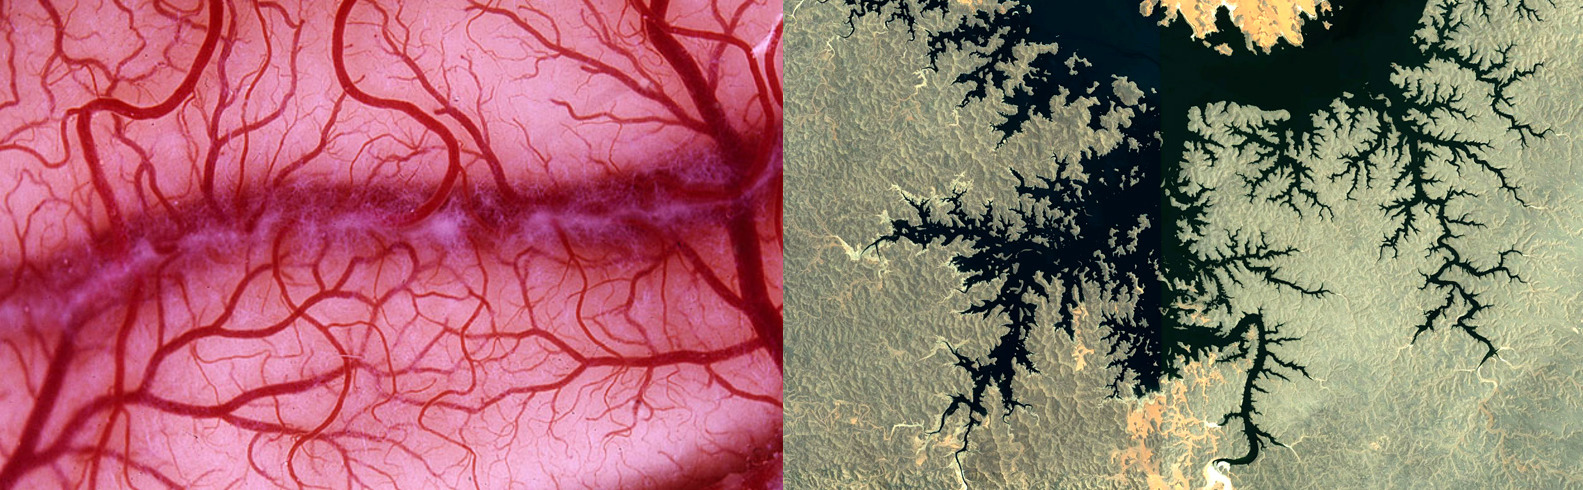
\includegraphics[width=.9\linewidth]{./out1.jpg}
\end{center}
\begin{center}
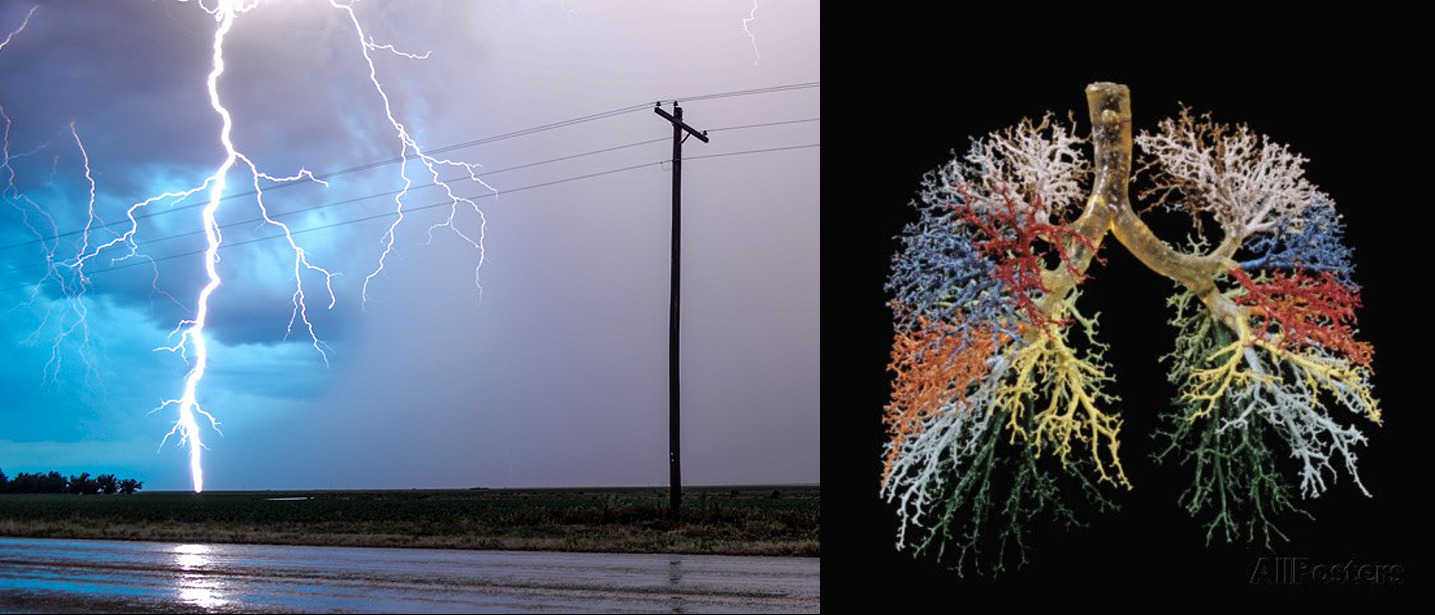
\includegraphics[width=.9\linewidth]{./out2.jpg}
\end{center}

\section*{Fractals: manufactured\ldots{}}
\label{sec:orgddda475}
\begin{center}
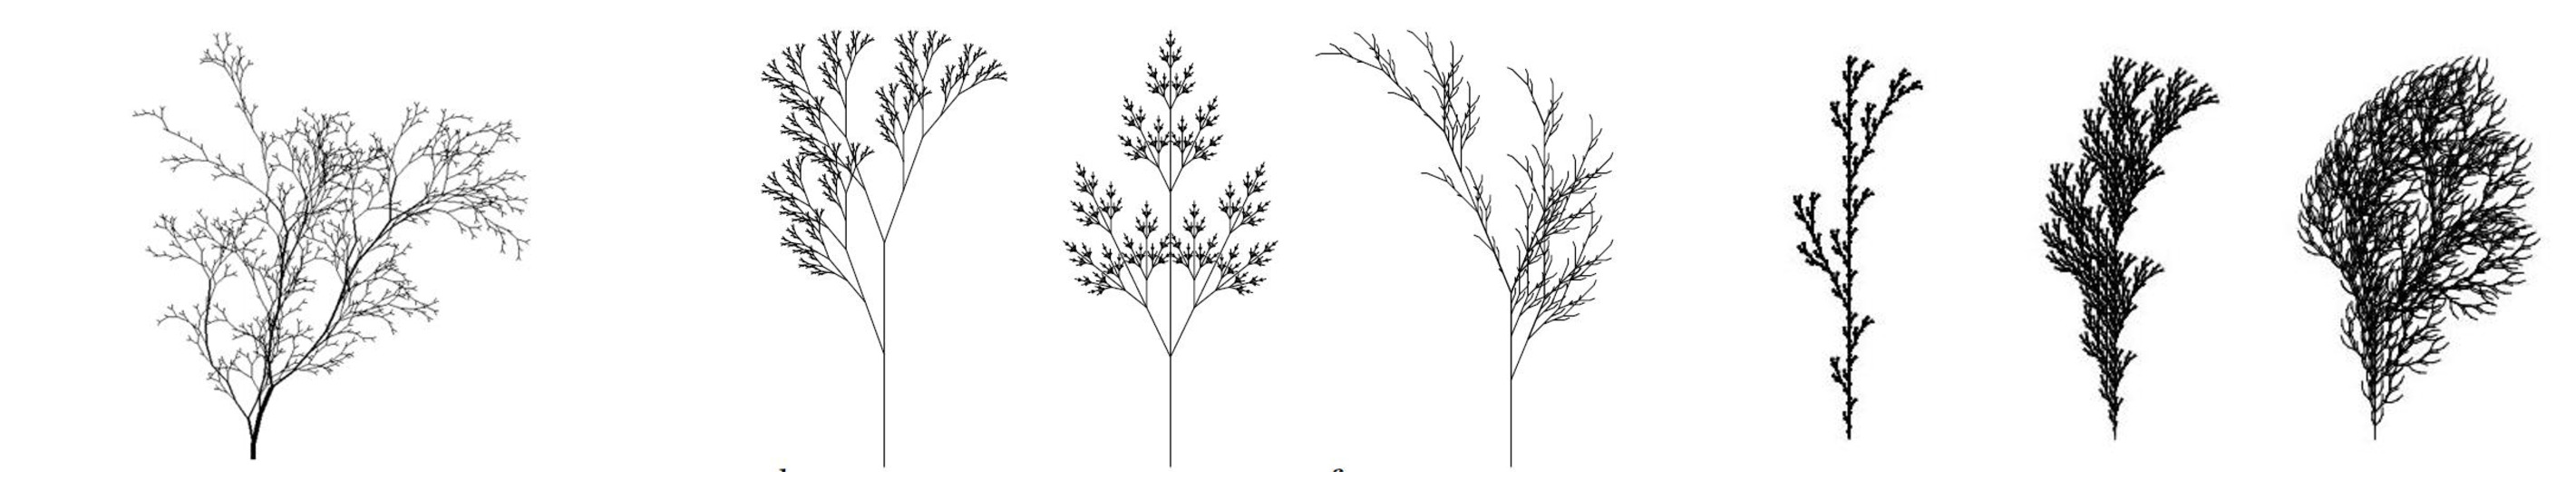
\includegraphics[width=.9\linewidth]{./agop.jpg}
\end{center}

These are all examples from \emph{The Algorithmic Beauty of Plants} by 
Aristid Lindenmayer and Przemysław Prusinkiewicz, available at 
\url{http://algorithmicbotany.org/papers/abop/abop.pdf}

\section*{Turning strings of symbols into pictures}
\label{sec:org2810c9d}

\begin{itemize}
\item Sets of rules describe how one string of symbols will be expanded to a new string
\item Each symbol corresponds to a \emph{turtle graphics} instruction:

\begin{itemize}
\item \texttt{F}: Move forward
\item \texttt{-}: Turn left
\item \texttt{+}: Turn right
\item \texttt{[}: Memorize current position and heading
\item \texttt{]}: Move to most recently memorized position and heading
\end{itemize}
\end{itemize}

\section*{An example}
\label{sec:org8056486}

For example, this sequence of symbols:

\texttt{F[+F]F[-F]F} 


has this output: 

We can clearly alter the output by changing the angle of the turns, 
and the length of the move forward.

In this example, the angle is 26\textdegree{}
\begin{center}
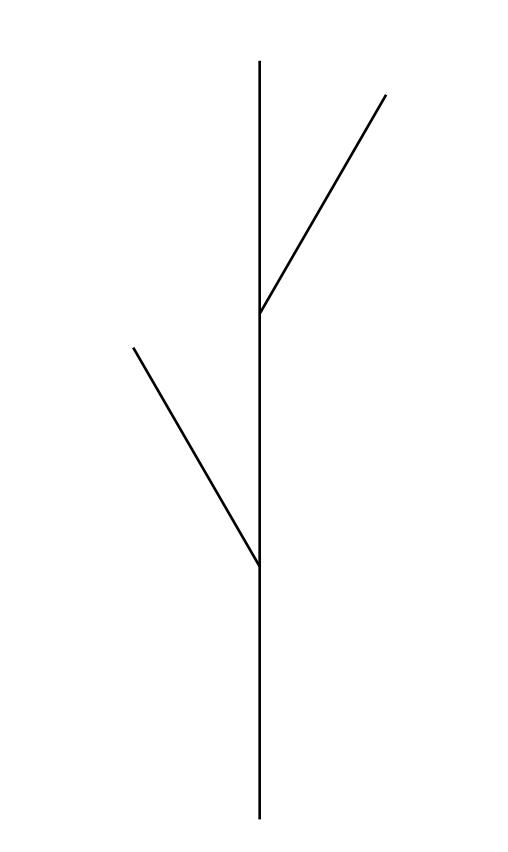
\includegraphics[width=.9\linewidth]{./l_tree1.jpg}
\end{center}

\section*{How turtle graphics works}
\label{sec:org33ef1d7}

This shows how the turtle draws a path with branches:

\begin{center}
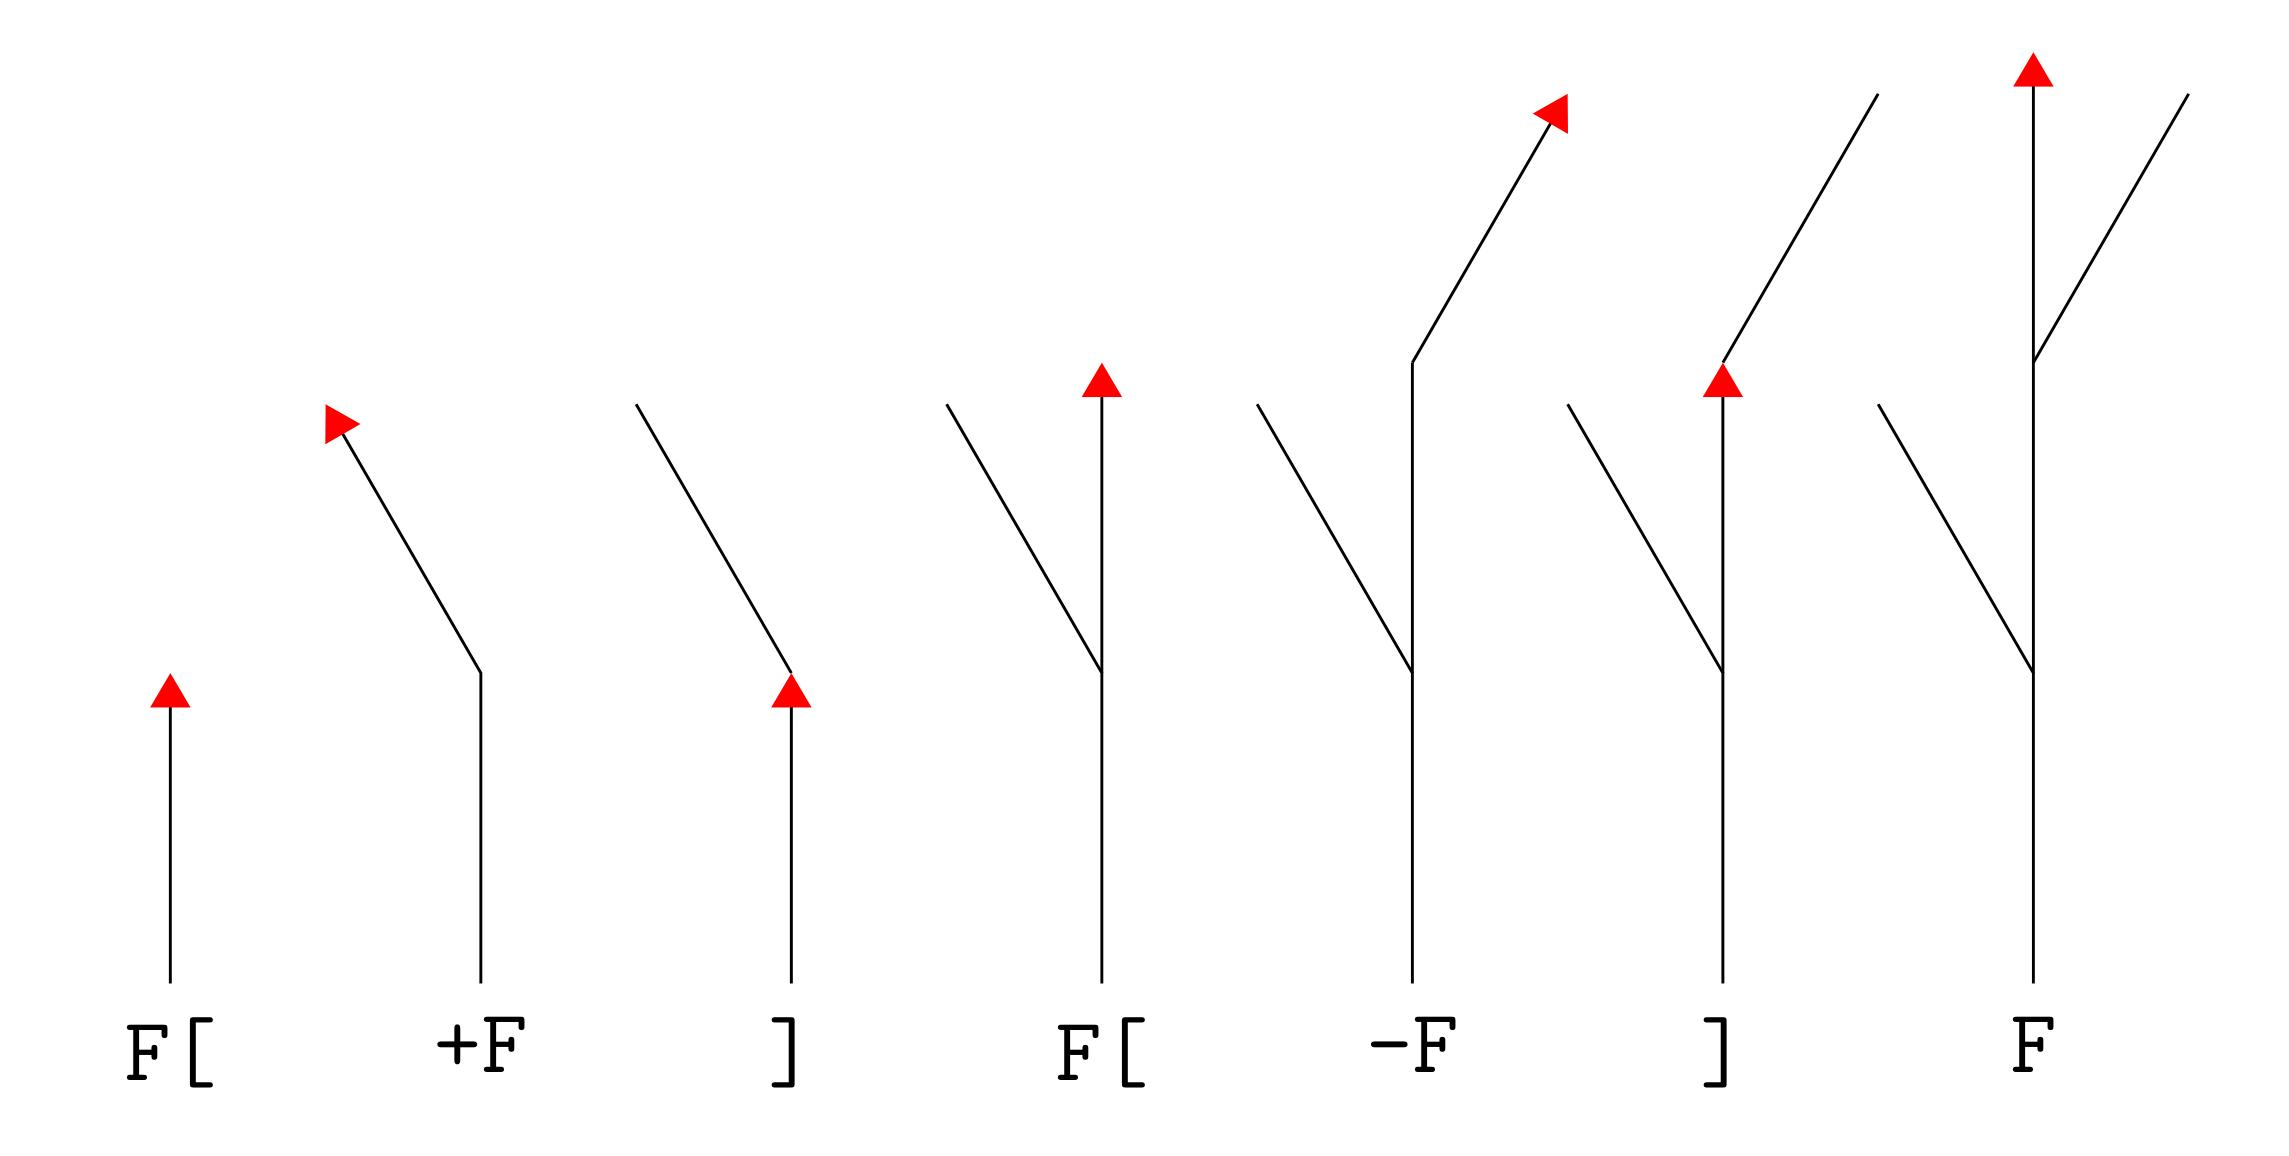
\includegraphics[width=.9\linewidth]{./growth.jpg}
\end{center}

\section*{More on turtle graphics}
\label{sec:orgcd1c995}

It's all done from the point of view of the turtle.  A side of \emph{Koch's
snowflake} can be computed by the rules:

\begin{itemize}
\item Start: \texttt{F}
\item Modify: \texttt{F} \(\rightarrow\) \texttt{F+F-{}-F+F} (with turns of 60\textdegree{})
\item At every further step, each \texttt{F} is replaced by the string \texttt{F+F-{}-F+F}
\item The second iteration produces

\texttt{F+F-{}-F+F+F+F-{}-F+F-{}-F+F-{}-F+F+F+F-{}-F+F}
\item The third iteration produces:

\texttt{F+F-{}-F+F+F+F-{}-F+F-{}-F+F-{}-F+F+F+F-{}-F+F+F+F-{}-F+F+F+F-{}-F+F-{}-F+F-{}-F+F+F+F-{}-F+F-{}-F+F-{}-F+F+F+F-{}-F+F-{}-F+F-{}-F+F+F+F-{}-F+F+F+F-{}-F+F+F+F-{}-F+F-{}-F+F-{}-F+F+F+F-{}-F+F}
\item and so on\ldots{}
\end{itemize}

\section*{Turtle graphics \emph{with pictures!}}
\label{sec:org4335b0d}


First iteration:~

Second iteration:~

Third iteration:~

Fourth iteration:~
\begin{center}
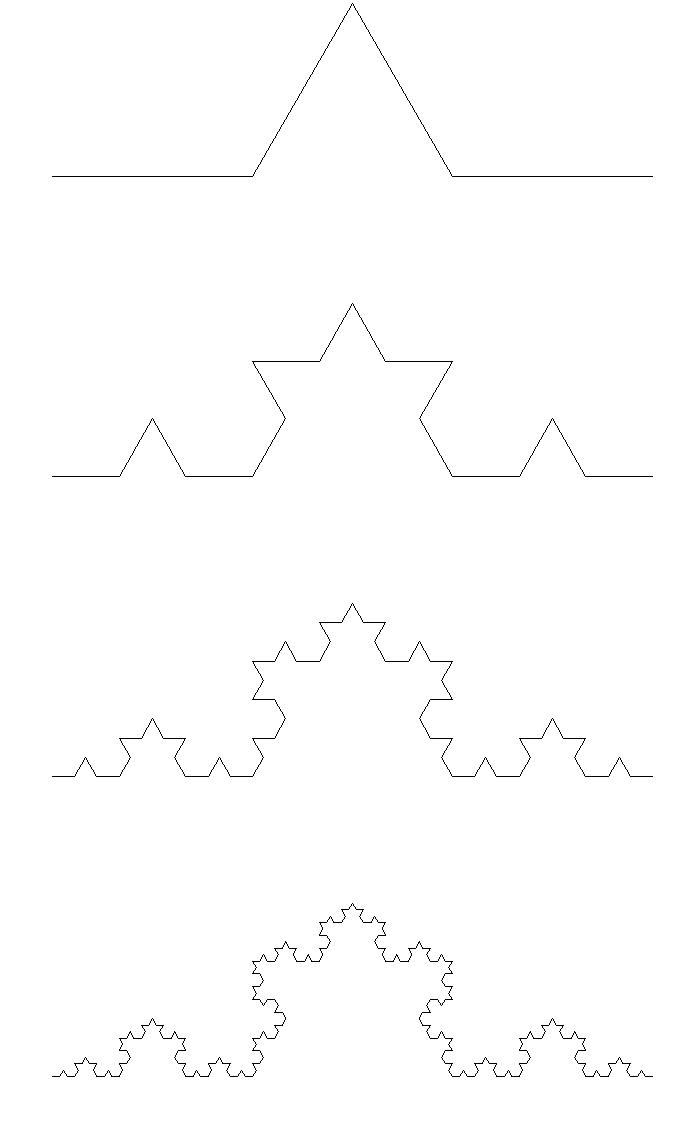
\includegraphics[width=.9\linewidth]{./koch_snowflake.jpg}
\end{center}

\section*{Some mathematics}
\label{sec:orge5165d4}

Remember the \texttt{F} \(\rightarrow\) \texttt{F+F-{}-F+F} iteration?  How many symbols 
are in the \(n^{\text{th}}\) string?

Let \(f_n\) be the number of \texttt{F}'s, and \(k_n\) be the number of other
symbols in the \(n^{\text{th}}\) string. We have:

\begin{eqnarray*}
f_{n+1}&=&4f_n,\quad f_1=4\\
k_{n+1}&=&4f_n+k_{n-1},\quad k_1=4
\end{eqnarray*}

It follows immediately that
\[
f_n=4^n\mbox{ and }k_n=4+4^2+4^3+\cdots+4^n=\frac{4}{3}(4^n-1).
\]
The total length is thus
\[
f_n+k_n=4^n+\frac{4}{3}(4^n-1)=\frac{1}{3}(7(4^n)-4).
\]


\section*{The fractal plant in modern languages: Python}
\label{sec:orgcd8cc98}

\begin{verbatim}
import turtle as t  # "turtle" is a turtle graphics module

# Lindenmayer system (a) from ABOP figure 1.24(a), p 25
def edgetree(level, size, angle):
    if (level==0):
	t.fd(size)
    else:
	edgetree(level-1, size/3, angle)
	t.lt(angle)
	edgetree(level-1, size/3, angle)
	t.bk(size/3)
	t.rt(angle)
	edgetree(level-1, size/3, angle)
	t.rt(angle)
	edgetree(level-1, size/3, angle)
	t.bk(size/3)
	t.lt(angle)
	edgetree(level-1, size/3, angle)
\end{verbatim}

\section*{The fractal plant in modern languages: Racket}
\label{sec:orgdd489e9}

Racket is a modern lisp; descended from Scheme.
\begin{verbatim}
;;   F -> F[+F]F[-F]F

(require furtle) ;; furtle is a simple but fast turtle graphics library
(: ltree_b (-> Real Real Real TurtleF))  ;; typed Racket so must declare types
(define (ltree level size angle)
  (if (= level 0)
      (turtles (forward size))
      (turtles (ltree (- level 1) (/ size 3) angle)               ; F
	       (save)                                             ; [
	       (left angle) (ltree (- level 1) (/ size 3) angle)  ; +F
	       (restore)                                          ; ]
	       (ltree (- level 1) (/ size 3) angle)               ; F 
	       (save)                                             ; [
	       (right angle) (ltree (- level 1) (/ size 3) angle) ; -F
	       (restore)                                          ; ]
	       (ltree (- level 1) (/ size 3) angle))))            ; F
\end{verbatim}

\section*{Some more mathematics}
\label{sec:orgf84faee}

\emph{Fractal dimension} can be defined by the "box-counting measure":

Suppose our picture is subdivided into boxes of size \(b\), and \(N(b)\) boxes 
are needed to cover the shape.  Its dimension can be defined as
\[
\lim_{b\to 0}\frac{\log(N(b))}{\log(1/b)}.
\]
For example, take a curve of length \(k\). As \(b\to 0\), we would find that
\[
N(b)\to \frac{k}{b}.
\]
Thus
\[
\lim_{b\to 0}\frac{\log(N(b))}{\log(1/b)}=\lim_{b\to 0}\frac{\log(k/b)}{\log(1/b)}
=\lim_{b\to 0}1-\frac{\log(k)}{\log(b)}=1.
\]
In general a fractal will have a non-integer dimension between 1 and 2.


\section*{The end}
\label{sec:orgd7afff7}

Thanks, folks!
\end{document}